\documentclass{article}

% Language setting
% Replace `english' with e.g. `spanish' to change the document language
\usepackage[swedish]{babel}
\usepackage{minted}
\usepackage{siunitx}
% Set page size and margins
% Replace `letterpaper' with`a4paper' for UK/EU standard size
\usepackage[a4paper,top=2cm,bottom=2cm,left=3cm,right=3cm,marginparwidth=1.75cm]{geometry}

% Useful packages
\usepackage{amsmath}
\usepackage{graphicx}
\usepackage[colorlinks=true, allcolors=blue]{hyperref}

\newcommand{\kursnamn}{Sensorer, AI och inbyggda system 4 hp}
\newcommand{\kurskod}{CC2018}
\newcommand{\provkod}{2201}

\begin{document}

%	Titelblad
\setcounter{page}{1}

  
\includegraphics[width=0.2\textwidth]{figures/HH_ENG_color_small.pdf}
	\begin{center}
	{\Huge{}Laboration 2 -- datainsamling och analys}
	\end{center}
\noindent\rule{\textwidth}{2pt}
\\


{\Large

\begin{tabular}{p{2cm}p{1cm}p{10cm}}
&  &  \\
Kurs: & 	& 	\kursnamn \\
Kurskod: & & \kurskod \\
Provkod: &  & \provkod \\
L\"arare: &  & Pererik Andreasson \& Fredrik Lundborg\\
\end{tabular}

% \vspace{10mm}
% \makebox[0.75\textwidth]{Namn:\enspace\hrulefill}

% \vspace{10mm}
% \makebox[0.75\textwidth]{Namn student 2:\enspace\hrulefill}

% \vspace{10mm}
% \makebox[0.75\textwidth]{Datum för genomförande:\enspace\hrulefill}

% \vspace{10mm}
% \makebox[0.75\textwidth]{Labbansvarig lärares signatur:\enspace\hrulefill}


}
\pagebreak

\tableofcontents

\section{Mjukstart med Anaconda och Jupyter}
I denna delen av kursen skall du göra några stycken datorlaborationer för att öka din förståelse av de verktyg som kan användas i datadrivna sammanhang. 
Samtliga övningar i detta häfte är obligatoriska för att få godkänt på kursen. Du behöver inte redovisa allt du har gjort, eftersom en del är övning för att komma igång, men vissa delar skall lämnas in som Powerpoint eller liknande och dessa är explicit markerade.

Dyker det upp frågor under ditt labbande ställ frågor i diskussionsforumet på Blackboard så svarar vi så fort vi kan.
\subsection{Börja med Jupyter}
Ladda ned Anaconda till din vanliga dator via följande länk:\\
\url{https://www.anaconda.com/products/individual}\\
I den här övningen skall vi öppna ett dataset och lära oss några funktioner i Python/Pandas för att lära oss något om vår data. Du kommer behöva ha Anaconda installerat på din dator för detta.  
\begin{enumerate}
\item Öppna Anaconda, bör se ut ungefär som på bilden nedan.\\
  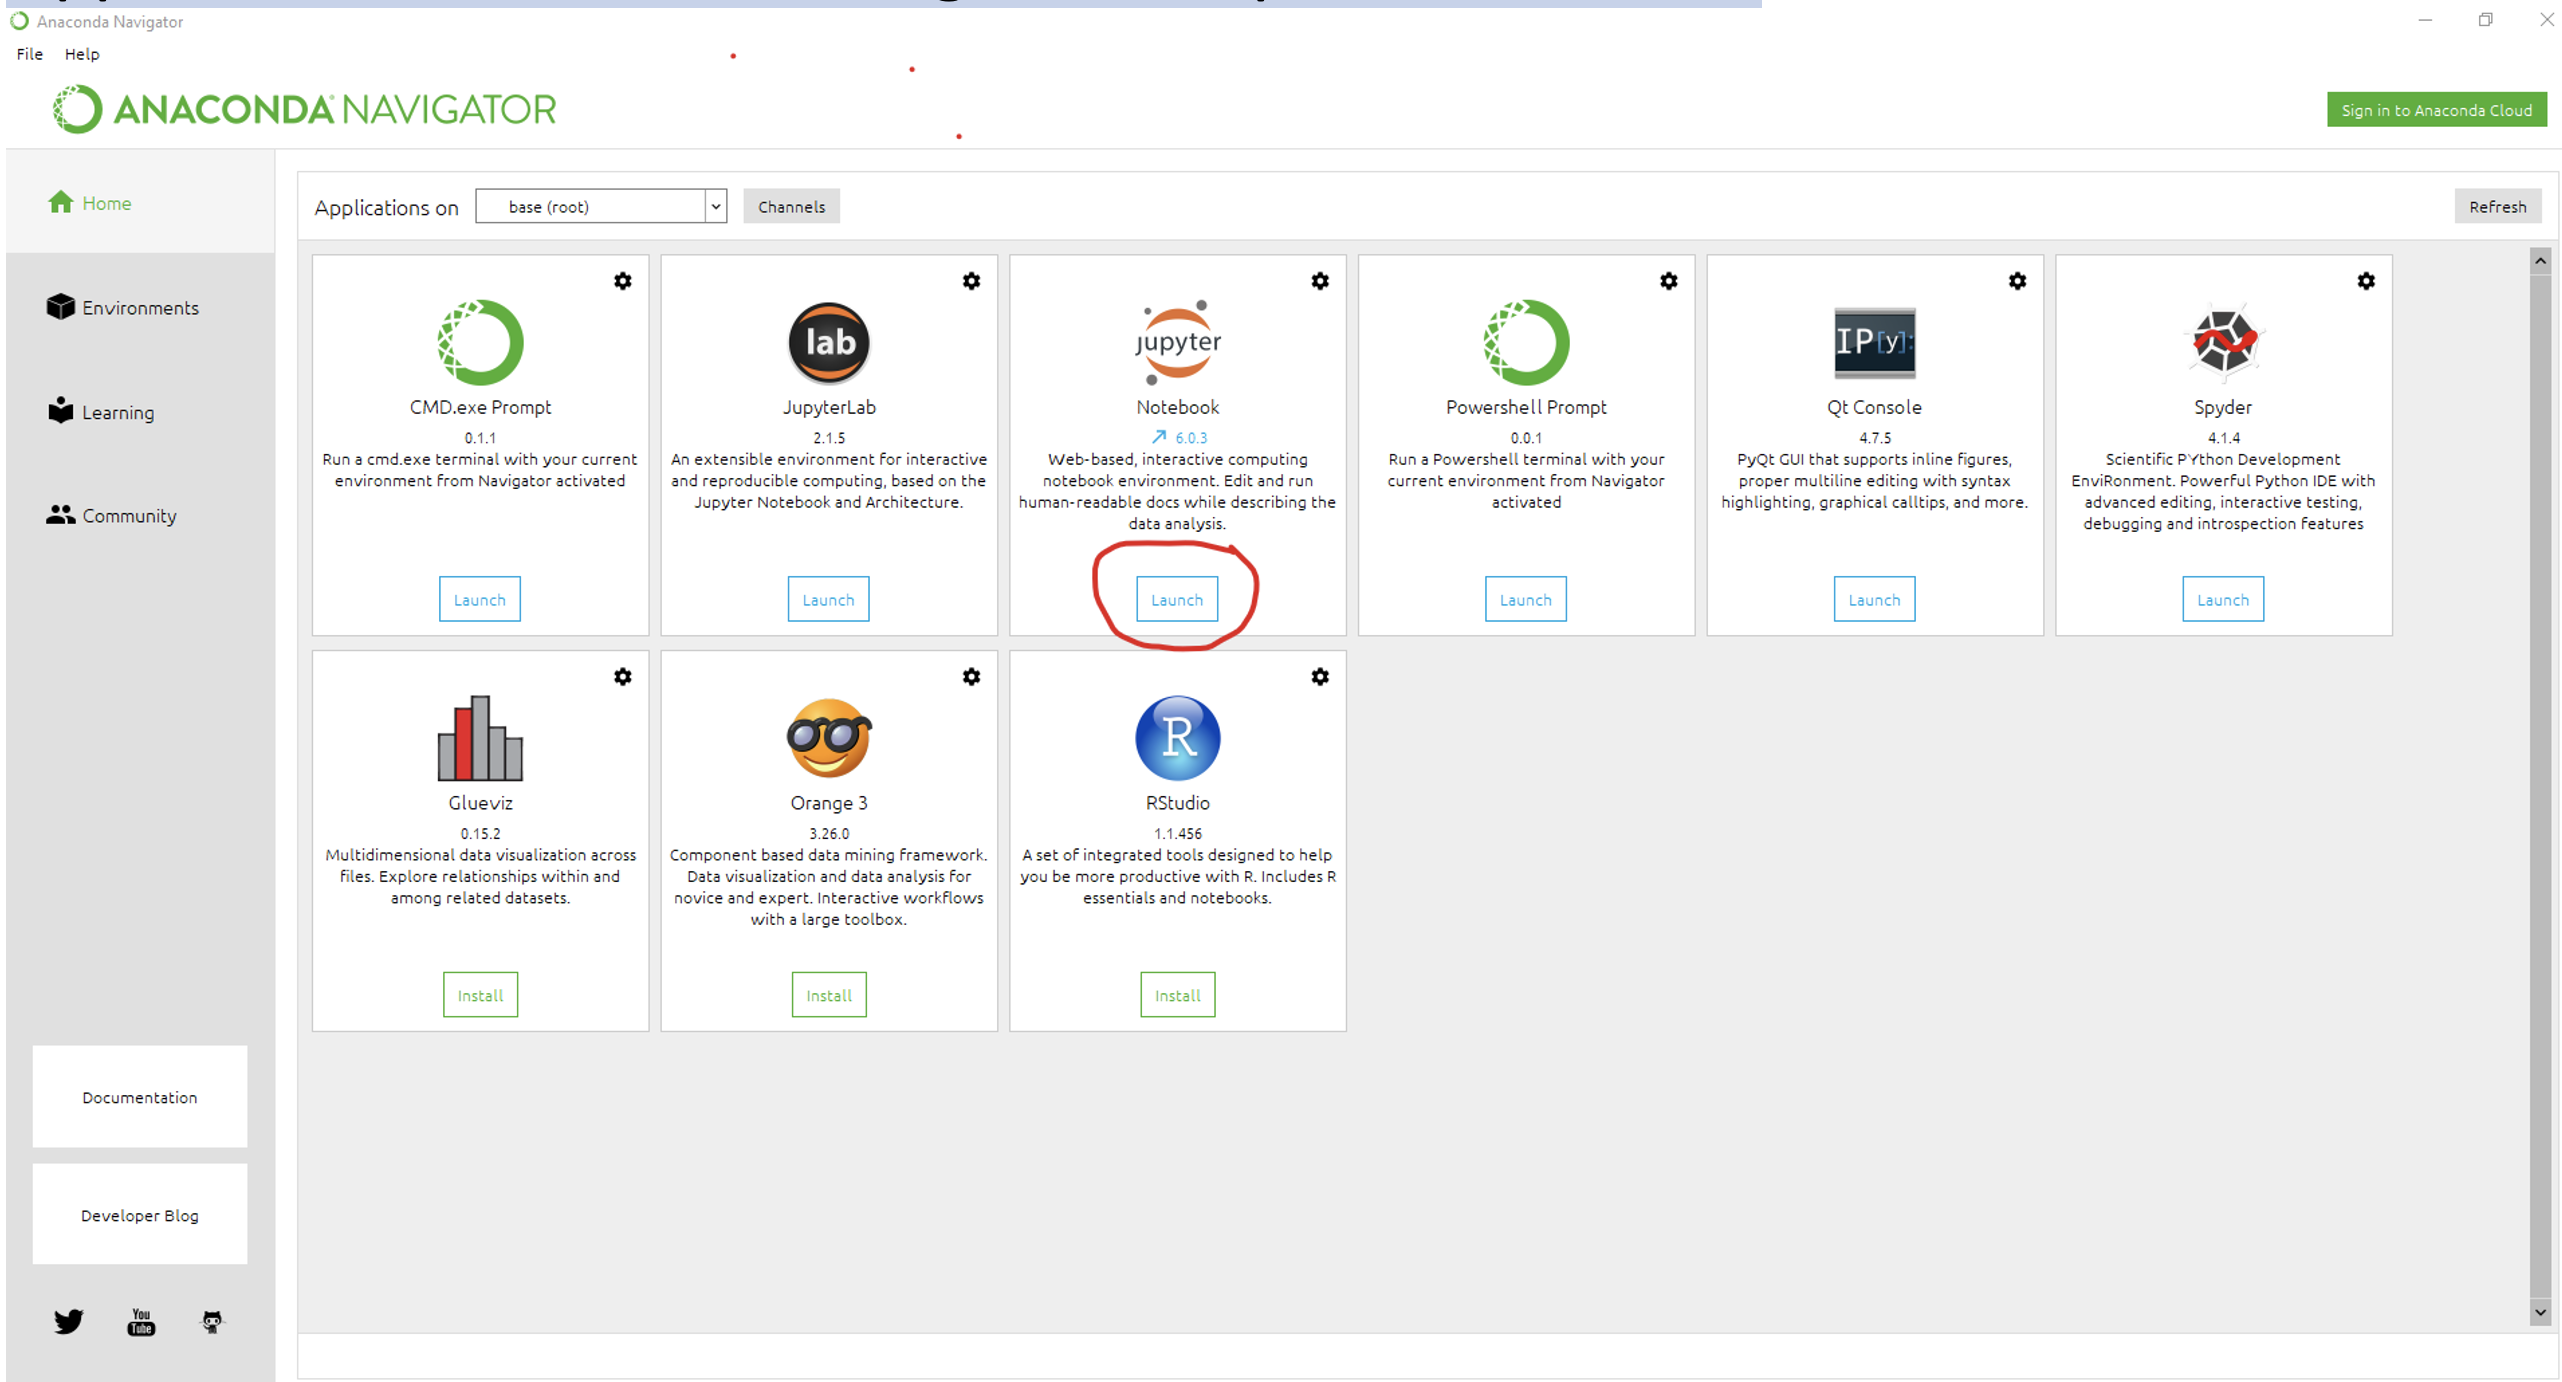
\includegraphics[width=\textwidth]{figures/anaconda1.png}
\item Starta Jupyter Notebook genom att trycka på \emph{Launch} som är inringat på bilden ovan. Då kommer det dyka upp en hemsida i din standardwebbläsare som ser ut ungefär som nedan.\\
  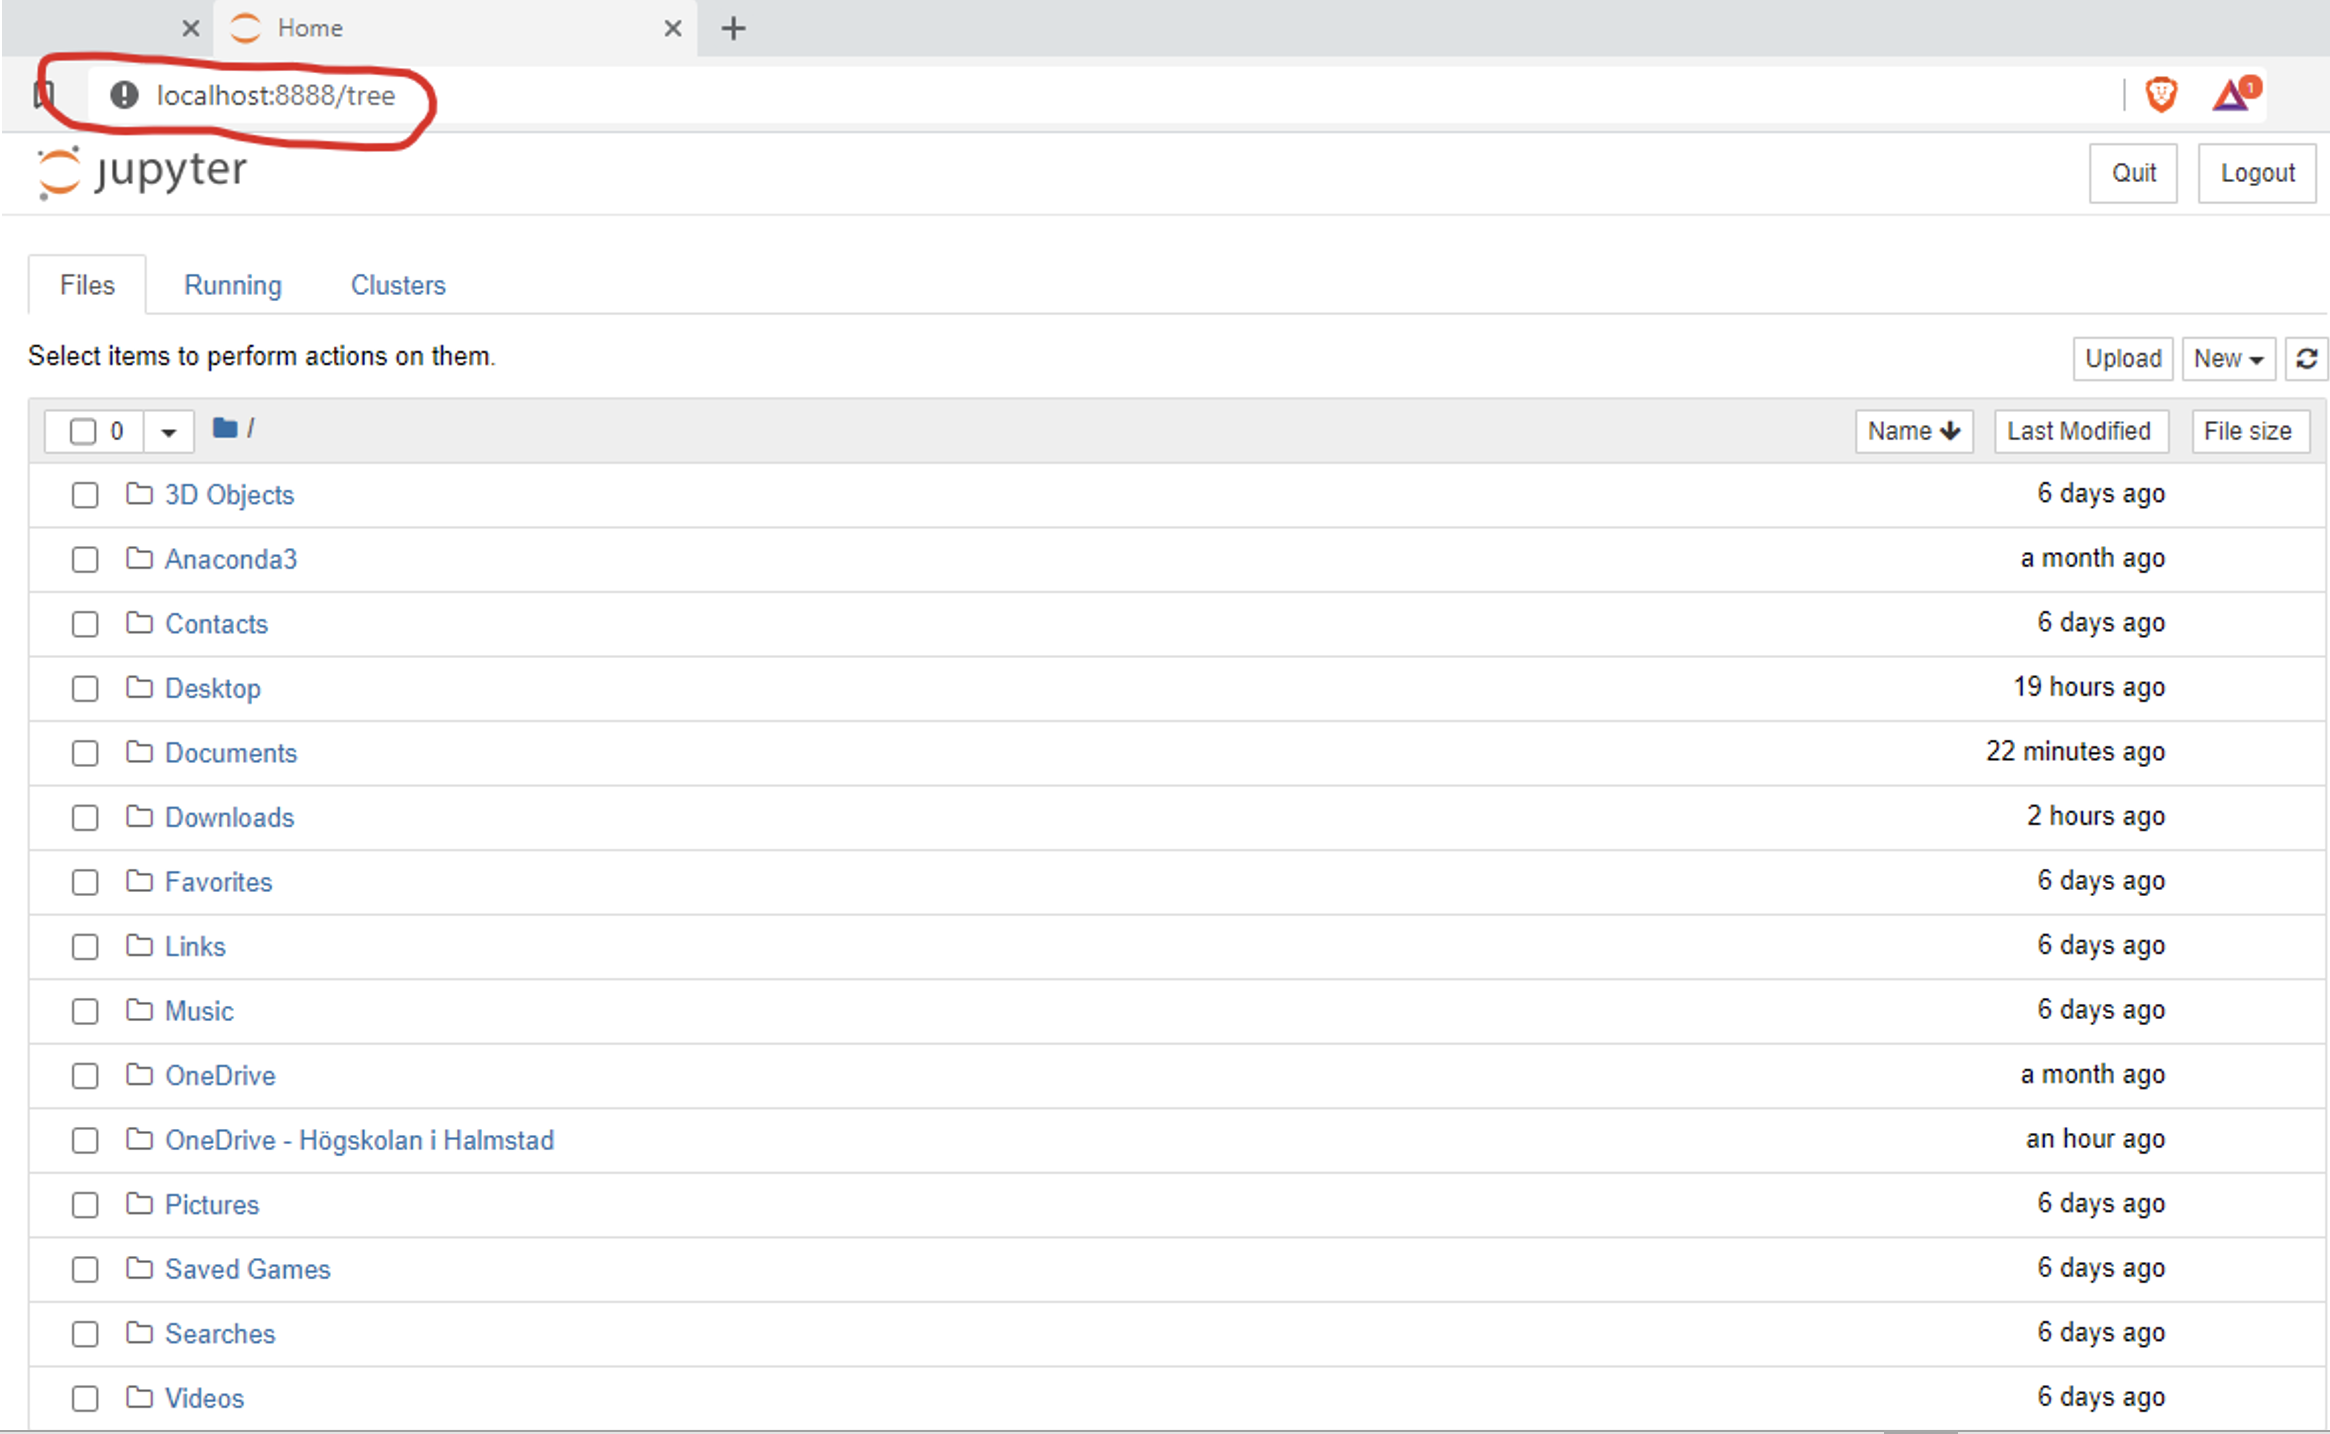
\includegraphics[width=\textwidth]{figures/anaconda2.png}\\
  Jupyter körs som en server på din dator, så du har nu med framgång loggat in som användare på denna server. Det som syns på bilden ovan är de filer och kataloger som finns i din hemkatalog, alltså på min dator det som finns i \verb+C:\Users\perand+, där \verb+perand+ är mitt användarnamn.
\item Skapa en ny katalog här genom att trycka på \verb+New+ uppe i högra hörnet och välj \verb+Folder+ för att skapa en ny katalog. Jupyter skapar en katalog som heter \verb+Untitled Folder+, vilket är lite oanvändbart. Markera check-boxen till vänster om katalognamnet och klicka på \verb+Rename+ för att döpa den till något mer användbart. Ett ganska bra namn är \verb+cc2018_labb2+. Klicka sedan på katalogen \verb+cc2018_labb2+ för att komma in i den. Det är här vi skall skapa och förvara de filer vi behöver under denna datorlaboration.
\item I Jupyter skall ni arbeta med \verb+notebooks+, det är ungefär dokument där det är möjligt att blanda Python-programmering med vanlig, beskrivande text, himla smidigt! Skapa nu din första Jupyter Notebook genom att igen välja \verb+New+ uppe i högra hörnet och välj sedan \verb+Python 3+ under \verb+Notebook+. Nu bör det ploppa upp en ny flik som ser ut ungefär som nedan.	\\
  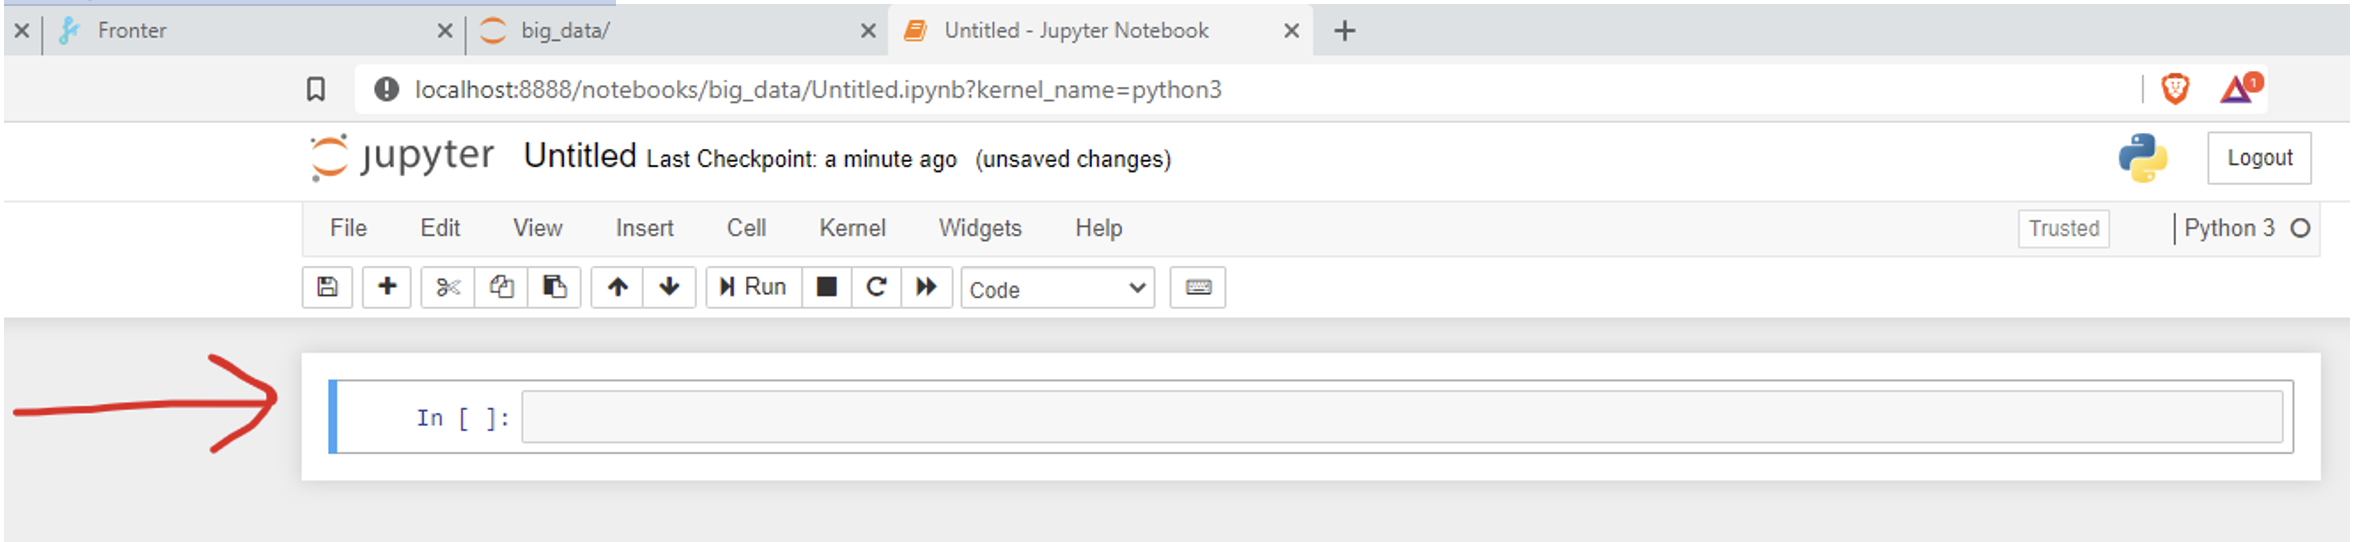
\includegraphics[width=\textwidth]{figures/anaconda3.png}\\
För att skriva och köra ditt första Pythonprogram i Jupyter, skriv
  \begin{minted}{python}
    print(''Hello Void'')
    \end{minted}
i rutan vid den röda pilen på bilden ovan. (Pilen är dit-ritad, den har ni inte i ert fönster.) För att sedan köra detta lilla program trycker du på knapparna Skift och Retur så exekveras det som är i denna ruta (eller \verb+cell+ som det kallas på Jupyter-språk). Bör se ut som nedan:\\
  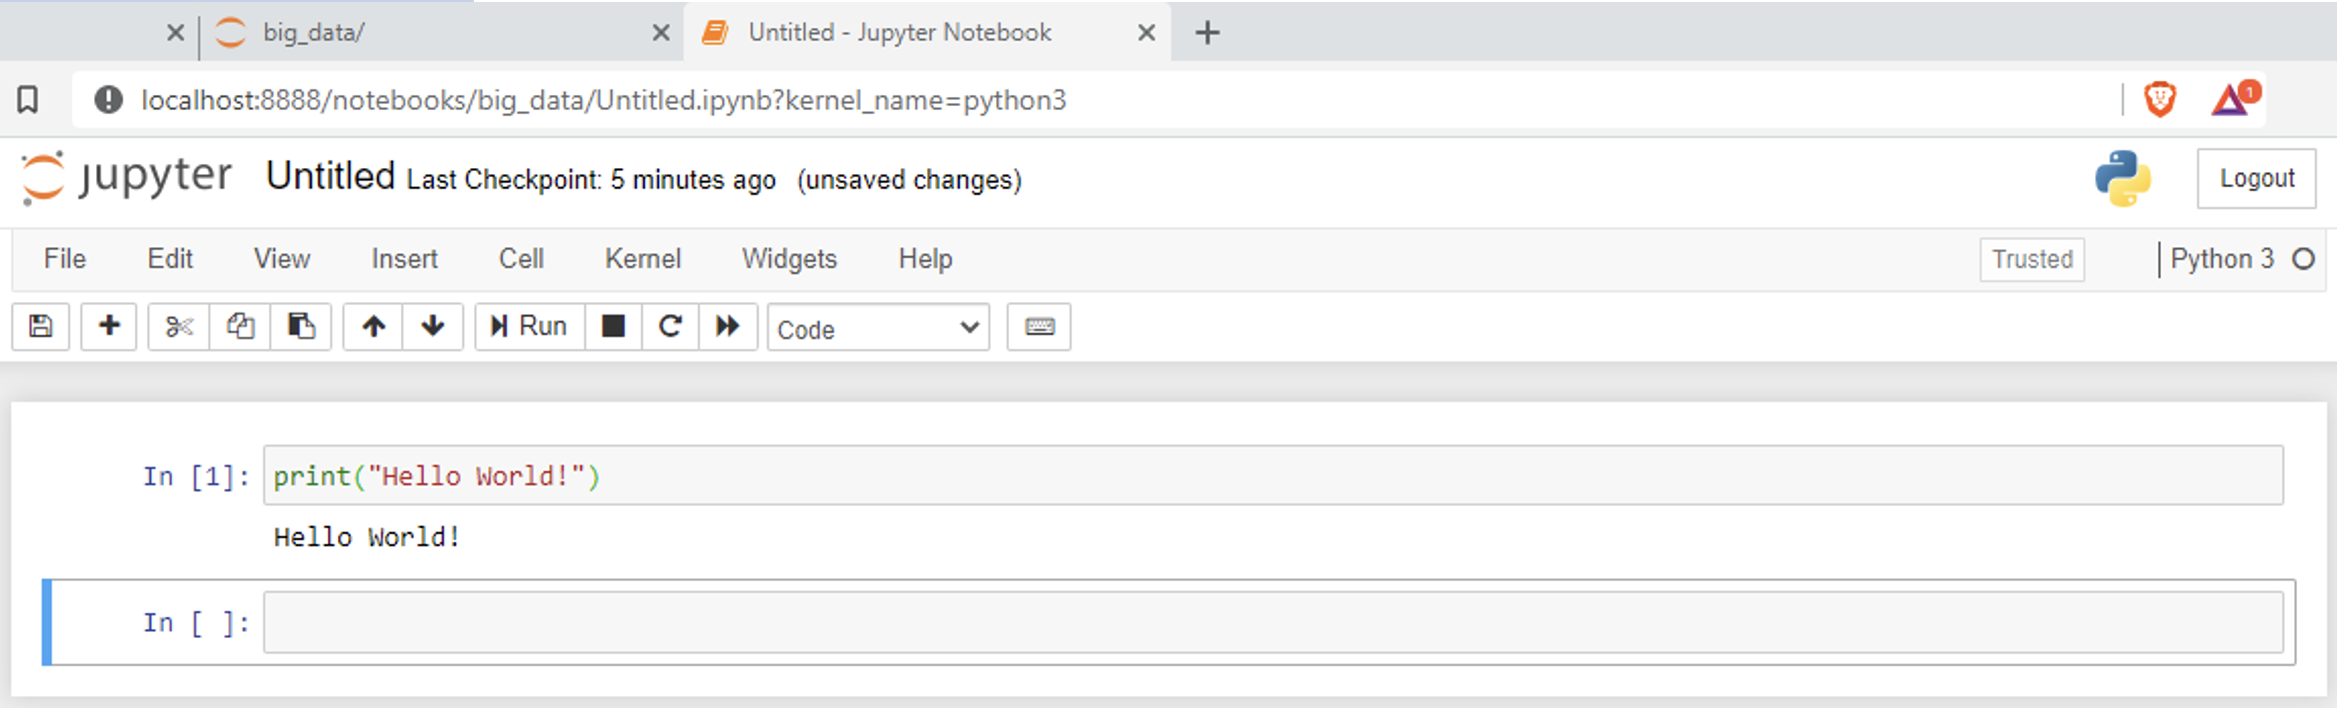
\includegraphics[width=\textwidth]{figures/anaconda4.png}
\item När vi körde programmet fick vi upp en ny cell där vi kan skriva andra saker. Om vi vill skriva text som inte skall behandlas som ett Pythonprogram behöver vi ändra om så att cellen är av typen \verb+Markdown+, det görs i den lilla rutan som är markerad i bilden nedan.	\\
  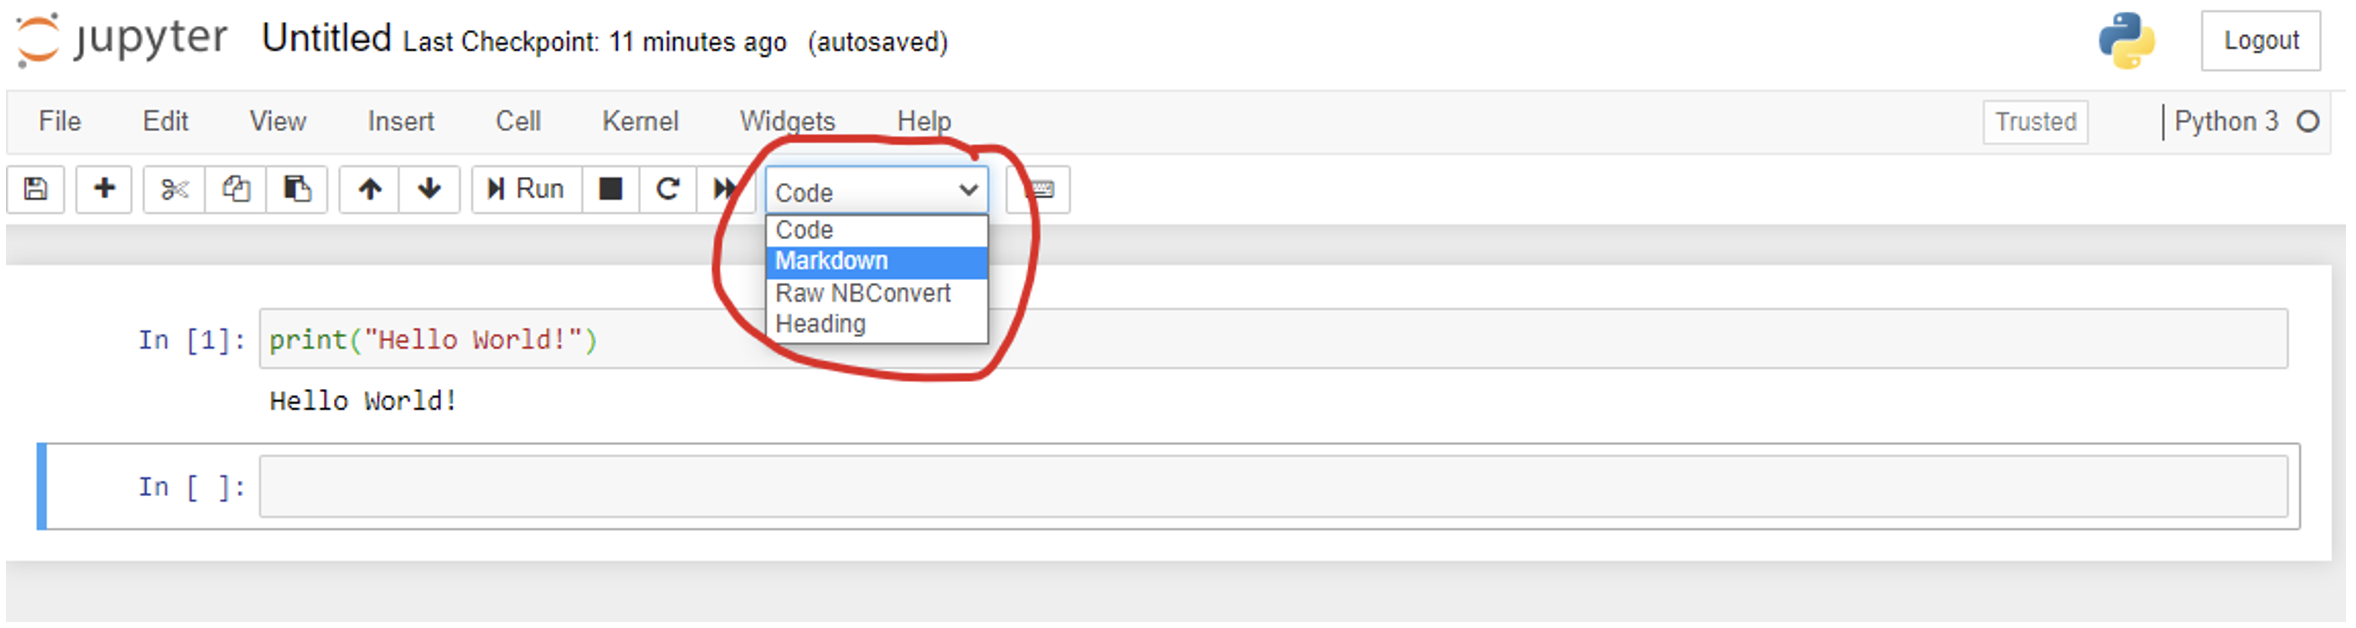
\includegraphics[width=\textwidth]{figures/anaconda5.png}\\
Nu kan vi skriva vad som helst i den rutan, till exempel lite information om att detta bara var ett testprogram. Allt som går som ”Markdown” eller ”Heading” struntar Python i. Test att skriva något i ”Markdown”-cellen! Kör sedan cellen genom att trycka på Skift och Retur så omvandlas det till snygg text och en ny cell ploppar upp, se nedan.
  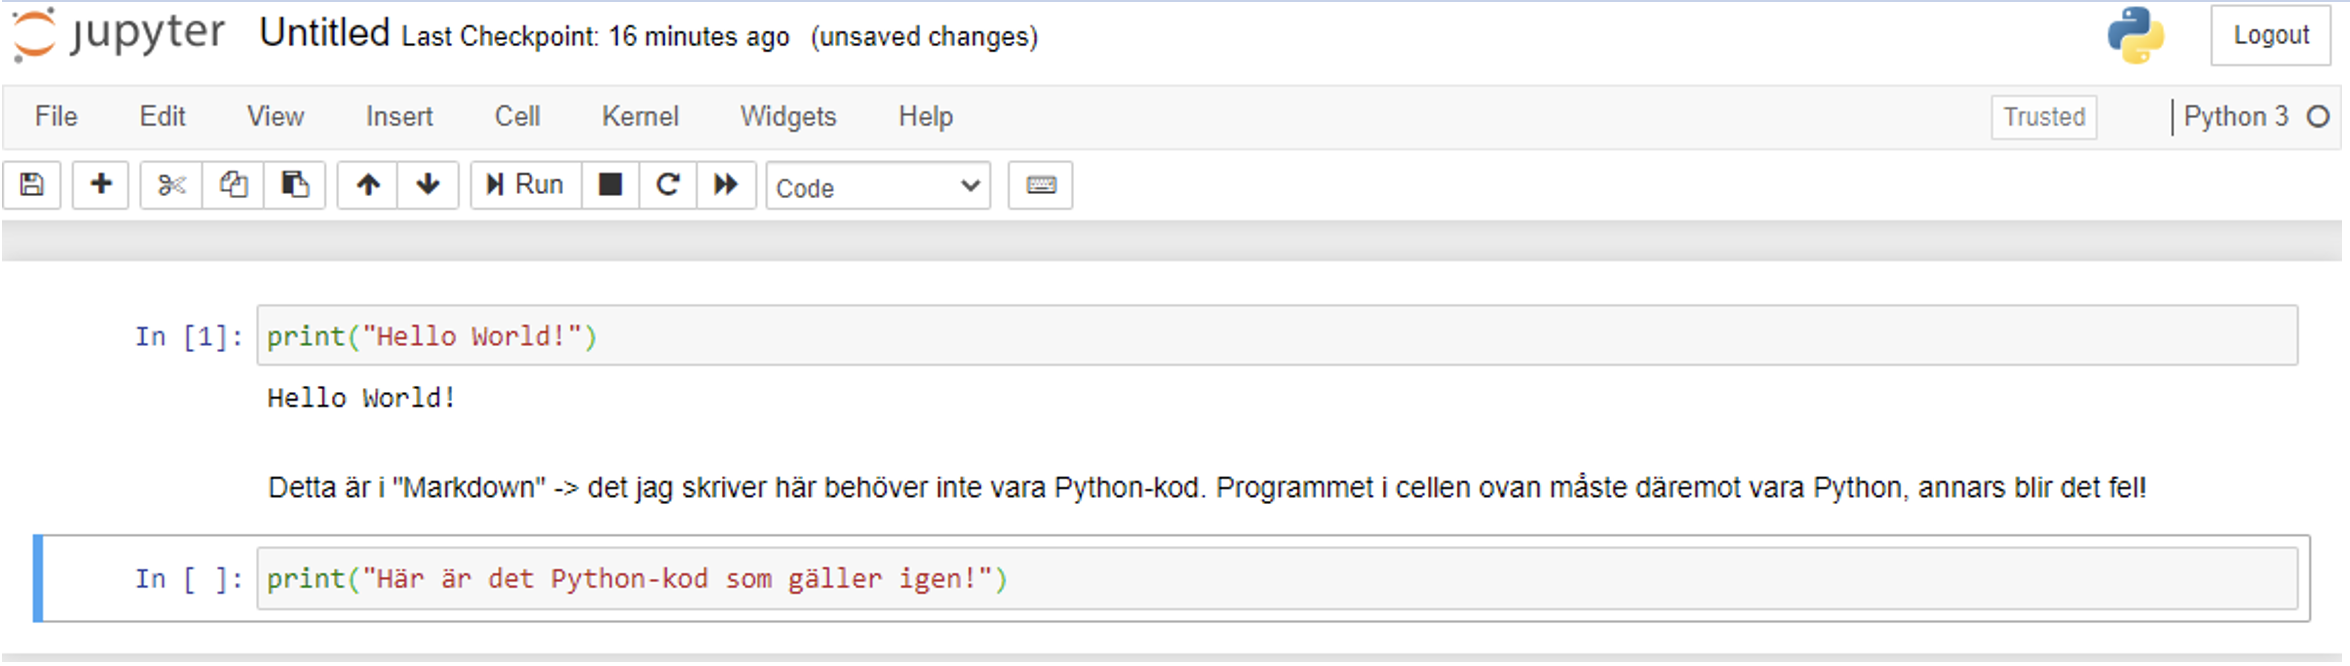
\includegraphics[width=\textwidth]{figures/anaconda6.png}\\
Det är lite påfyllt med Pythonkod i cellen nedanför.
\item För att döpa om din Notebook, klicka på \verb+Untitled+ längst upp och hitta på ett trevligt och informativt namn, ex \verb+cc2018_lab2+.\\
  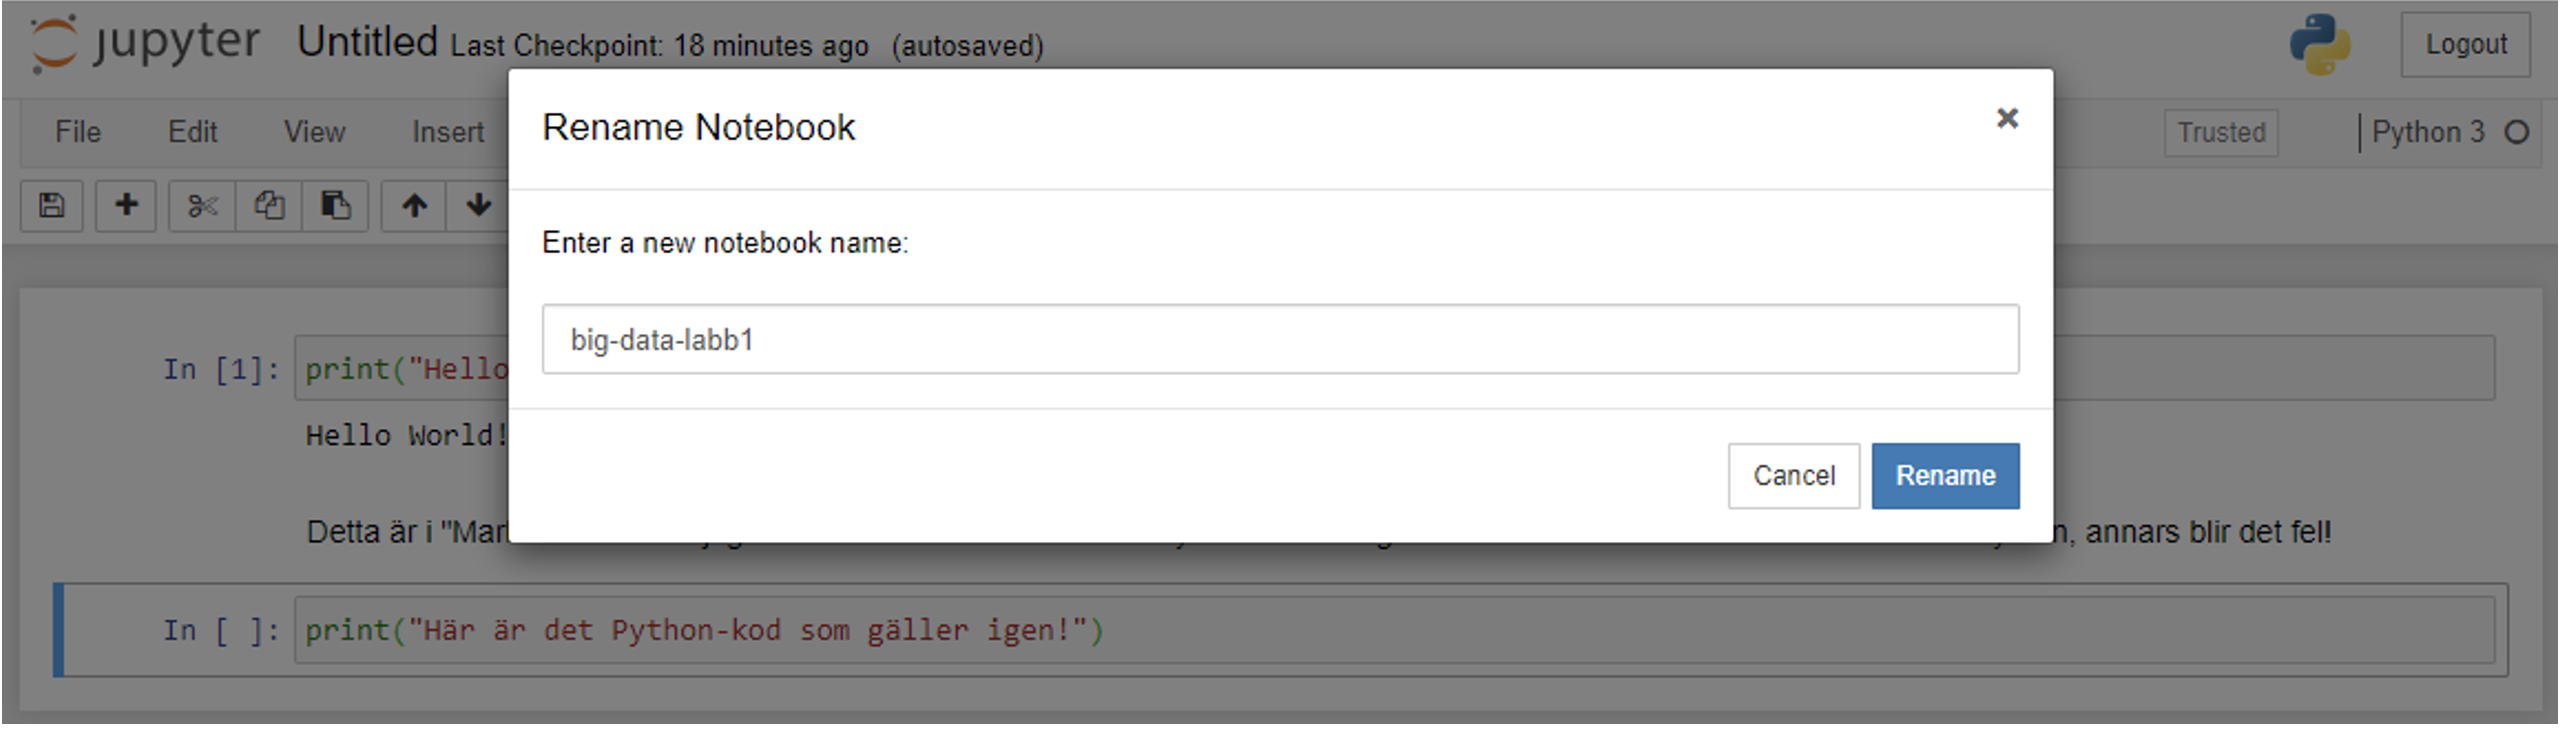
\includegraphics[width=\textwidth]{figures/anaconda7.png}\\
  \end{enumerate}

\textbf{OBS:} Viktigt är att om du stänger av Jupyter och öppnar din notebook vid senare tillfälle måste du köra alla celler för att data skall laddas in igen. Om du öppnar på nytt och det strejkar, kör alla celler genom att välja \verb+Cell+-menyn och välj \verb+Run all+ så körs alla celler och du är åter på banan. Då är det viktigt att alla celler är körbara, så undvik att lämna celler som genererar felmeddelanden i din notebook.

\textbf{OBS:} Vid början på varje cell i en notebook blir det ett tal när du kör den, den första blir 1, den andra 2, osv. Dessa tal är för att hålla ordning på i vilken ordning cellerna har körts, kan vara bra att veta när något försvinner som förut fanns där etc. En cell nedanför en annan cell kan således vara \emph{äldre} än den övre och ha skrivits över av en cell ovanför.

\subsection{Ladda in data med Pandas}
Data som ni skall använda i den här övningen är mina stegdata för 2020, ladda ner filen\\ \verb+Steg2020_Pererik.csv+ som ligger i samma katalog på Blackboard som denna Laborationsanvisning. För att övningen nedan skall fungera måste stegdatafilen ligga i samma katalog som din Jupyter notebook, enligt ovan alltså för mig i katalogen \verb+C:\Users\perand\big_data+. Målet med denna övning är att känna lite på Pandas och att få fram en steg-rekommendation baserat på detta, alltså hur många steg  per dag som är rekommenderade. Stegmålet bör vara ett mål som kräver lite ansträngning för att uppnå, t.ex. om genomsnitt är 10000 steg per dag, kanske ett mål att arbeta mot är något över, 11000 eller 12000. 
%Now trying \mintinline{python}{print(''Hello Void!'')} to see how that rocks!
% \mintinline{python}{}

Vi har i kursen träffat olika typer av \emph{moduler} som kan laddas in i Pythonprogram som utökar funktionaliteten, hittills har vi träffat både modulen \verb+time+ och \verb+network+ till exempel. I denna del skall vi använda en modul som heter \verb+pandas+ och importerar vi denna fungerar det ungefär som Excel fast Python. För att läsa in data med \verb+pandas+ måste vi först importera \verb+pandas+-modulen. 
\begin{enumerate}
    \item Börja en ny cell i din Jupyter notebook och skriv \mintinline{python}{import pandas as pd} överst i den cellen. Detta skall vara utan radindrag. För att använda funktionalitet från Pandas skriver vi modulnamnet, pd, direkt följt av en punkt och direkt följt av namnet på den funktionen vi vill använda. För att läsa in tabelldata från vanligt textformat skall vi använda funktionen \mintinline{python}{pd.read_csv()} där \verb+csv+ står för \emph{comma separated values}. 
    \item I \verb+Steg2020_Pererik.csv+ är kolumnerna i tabellen separerade med semikolon, så vi måste säga detta till Pandas, för att läsa in mina stegdata, skriv på raden under i din notebook cell:
  \begin{minted}{python}
    stegdata = pd.read_csv("Steg2020_Pererik.csv", sep = ";")
    \end{minted}
Här kallar vi den inlästa data (är en variabel på Pythonspråk) \verb+stegdata+. \mintinline{python}{sep = ”;”} anger att det är semikolon som separerar kolumner från varandra. Kör du denna cell laddas stegdatan in och du kan komma åt den genom att använda variabeln \verb+stegdata+. 
\item \textbf{Titta på tabellhuvudet.} Med kommandot \mintinline{python}{stegdata.head()} efter att du laddat in stegdatan så visar Jupyter de fem första raderna av tabellen på ett välkänt och snyggt sätt. Observera att väl inladdad är \verb+stegdata+ ett Pandas-objekt (en \verb+dataframe+ för att använda Pythonspråk) så vi kan komma åt Pandas funktioner genom att använda punkt efter variabelnamnet. Kör du cellen bör du få upp ungefär som nedan:\\
  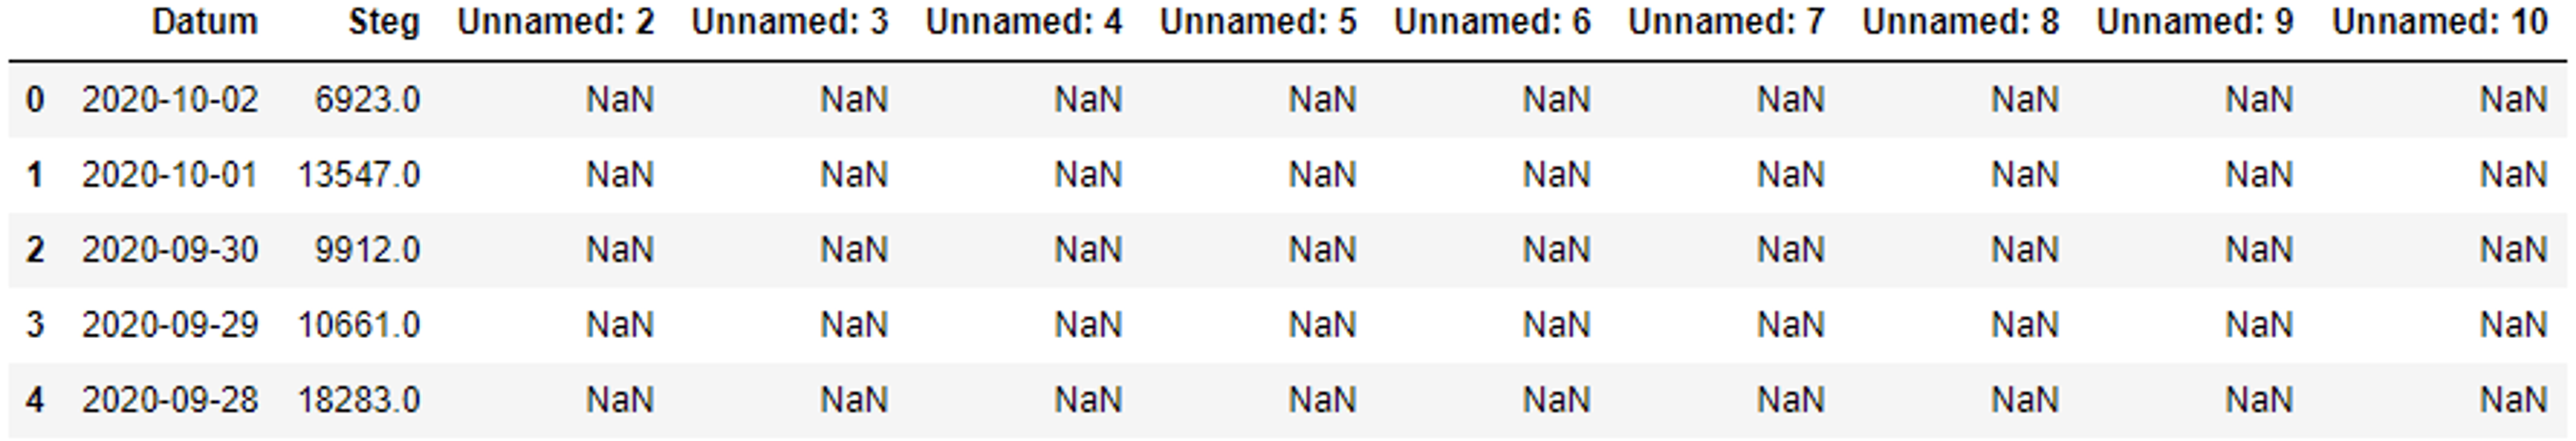
\includegraphics[width=\textwidth]{figures/anaconda8.png}\\
Här ser vi från vänster till höger radnummer, datum, antal steg för den dagen följt av nio kolumner som innehåller \verb+NaN+ (Not a Number) pga att mina stegdata innehåll en massa semikolon på varje rad (pga ful export från Excel).
\item \textbf{Snabb statistik på stegdatan.} Testa kommandot \mintinline{python}{stegdata.describe()}  så får vi fram lite mer information om stegdatan. Bland annat hur många datapunkter vi har (hur många dagar som har en stegdatapunkt, skall vara 271), minsta och största värde, medelvärde etc. Om du tittar på minsta värde är detta 0, vilket känns felaktigt eftersom det är nästan omöjligt att gå noll steg.
\item \textbf{Städa upp i datan 1.} För att kunna gå vidare med någon form av dataanalys behöver data alltid städas upp lite. Vi skulle kunna t.ex. ta bort de kolumner som inte innehåller någon data, d.v.s. kolumnerna som heter \verb+Unnamed: 2 – 10+. Det finns jättemånga olika sätt att göra detta, lättast att förstå är att vi använder kommandot \verb+columns+ för att välja kolumner. Med raden nedan gör vi en ny variabel där vi sparar den nya tabellen som bara innehåller datum och steg:
\begin{minted}{python}
stegdata_liten = stegdata[stegdata.columns[[0, 1]]]
\end{minted}
(Ledsen för alla hakparenteser, men sånt är livet.) Om vi sedan testar \mintinline{python}{stegdata_liten.head()} ser vi att vår nya \verb+dataframe+ bara innehåller två kolumner, datum och antal steg för den dagen. 
\item \textbf{Städa upp i datan 2.} Som påpekades ovan är dagar med noll steg nästan omöjliga, därför behöver vi behandla dagar med noll (eller dagar med väldigt få steg) på något sätt så de inte påverkar statistiken på ett felaktigt sätt. Det finns flera sätt att angripa detta, lättast är att vi hittar de datum som har noll steg och tar bort dessa dagar ur datan. Raden nedan kommer avslöja vilka datum som har noll steg registrerade:
\begin{minted}{python}
stegdata_liten[stegdata_liten["Steg"]==0]
\end{minted}
Här använder vi funktionen \verb+loc+ som lokaliserar, eller hittar, data som uppfyller vissa villkor. I det här fallet uppfyller det villkoret att Steg-kolumnen innehåller en nolla. För att ta bort dessa rader kan vi använda funktionen \verb+drop+, säga till den vilka rader (från kommandot ovan), säga att vi menar rader (\verb+axis = 0+ ger rader och \verb+axis = 1+ ger kolumner) och undvika att göra en ny kopia (\verb+inplace = True+):
\begin{minted}{python}
stegdata_liten.drop([19, 58, 127, 202], axis = 0, inplace = True)
\end{minted}
Testar vi igen kommandot ovan som ger alla noll-värden kommer det, förhoppningsvis, komma upp tomt. Kör vi \verb+drop+-kommandot igen blir det fel eftersom dessa rader saknas då i \verb+dataframe+:en. Givetvis går det bra att spara raderna som en variabel för att snygga till det (och då går det att köra kommandot igen utan fel). 
\item \textbf{Städa upp datan 3.} Kör vi \verb+describe()+-funktionen på vårt nya, städade dataset ser vi att vi har färre värden (de fyra vi tog bort i förra steget) och att medelvärdet har stigit något. Vi ser att minsta värdet har ökat från noll till ett värde som igen är orimligt, det finns inga dagar som Pererik har tagit så få steg. För att utesluta dessa dagar med väldigt få steg (men fler än noll) återanvänder vi vårt kommando från ovan \emph{men ändrar villkoret}. Här är det lite godtycke inblandat, men en gissning är att dagar med färre än 4000 steg så har antingen batteriet i min stegmätare tagit slut eller så har något extraordinärt hänt. Vi kör kommandot:
\begin{minted}{python}
stegdata_linten.loc[stegdata_liten["Steg"]<4000]    
\end{minted}
Här dyker det upp åtta fall, där vissa är speciella. Här kan det ha varit dagar som Pererik varit sjuk eller liknande, men högst sannolikt är att batteriet har tagit slut. Testa att öka från 4000 i lite olika steg och se vad som händer. En bra gissning (har testat lite) är att ungefär färre än 4000 steg hör till extrema ovanligheter. För att ta bort dessa ur stegdatan gör vi som för borttagandet av noll, vi använder \verb+drop+ på de index som vi fick från \verb+<4000+-kommandot:
\begin{minted}{python}
stegdata_liten.drop([20, 69, 154, 183, 208, 214, 215, 222], 
                    axis = 0, inplace = True)
\end{minted}
Igen går det givetvis bra att spara dessa (dagar med färre än 4000 steg) som en variabel så att kommandot kan köras flera gånger. Tittar vi igen på stegdatan med \verb+describe()+ bör medelvärdet ha ökats något ytterligare. Om vi tittar lite noggrannare på datan så ger \verb+describe()+ nu att vi skall ha 259 steg-datapunkter, men om vi kollar på längden av hela tabellen har den 264 rader (kan kollas med kommandot \verb+shape+, som i \mintinline{python}{stegdata_liten.shape}). De fem ”datapunkter” innehåller inga värden, och kan tas bort med funktionen \verb+dropna()+, så för att fullända vår rensning av datan bör det sista vi gör innan vi kan besluta hur många steg Pererik skall ha som mål att ta per dag vara att ta bort dessa tomma datapunkter. Om vi kallar det en ny variabel (här \verb+stegdata_ren+) kan det göras med kommandot:
\begin{minted}{python}
stegdata_ren = stegdata_liten.dropna()
\end{minted}
Om vi använder \verb+shape+ och \verb+describe()+ efter detta ser vi att vi nu har rätt antal datapunkter. Dessa tomma datapunkter bidrog inte till statistiken från \verb+describe()+, så att ta bort dessa förbättrar inte vår förståelse i nuläget. Om vi skall använda datan till någon mer avancerad analys hade dessa punkter kunnat ställa till problem.
\item \textbf{Slutkläm på stegdata.} I redovisningen av denna uppgiften (det som skall in på din Powerpoint-presentation) skall du klippa in vad kommandot \verb+describe()+ ger efter din data-rensning från ovan samt ett lämpligt stegmål baserat på hur många steg Pererik tar i genomsnitt per dag. Skaffa gärna lite källor på lämpliga stegmål och knyt an din rekommendation till dessa.
\end{enumerate}
\subsection{Väderdata –- Medeltemperatur i juli}
Under den här övningen skall vi öva på att utforska data som finns tillgängligt öppet för vem som helst att använda. Det finns väldigt många olika källor som har varierande kvalitet. I den här övningen skall vi använda SMHIs väderdata för att bestämma medeltemperaturen i juli för de senaste åren så nära vårt hem som möjligt. Så nära som möjligt menas att SMHI inte har väderstationer överallt, så det gäller att hitta den väderstation som är närmst ditt hem.
\begin{enumerate}
    \item Data brukar hämtas från så kallade APIer, API står för \emph{Application Programming Interface} och är en tjänst som något datorprogram erbjuder andra datorprogram för att komma åt resurser i det första datorprogrammet.\footnote{Överkurs: skriv ett Pythonprogram som laddar ner direkt från SMHI:s API!} Alltså: för att olika program skall kunna kommunicera med varandra. Verkar det luddigt? Det är det, men i vårt fall kommer SMHIs API att behandlas i stort sett som en hemsida där vi laddar ner väderdata. För att komma åt SMHIs API via din webbläsare:
    \begin{enumerate}
        \item Surfa in på \url{https://www.smhi.se/}
        \item Klicka på \textbf{Data}, välj \textbf{Meteorologi} och välj \textbf{Temperatur}.
        \item På \textbf{Temperatur}-sidan, klicka på länken \textbf{Lufttemperatur, timvärde}
        \item Det dyka upp en karta med SMHIs alla väderstationer, zooma in och titta runt tills du hittar den station som ligger närmst ditt eget hem. Tänk på att välja en aktiv station, för mig är den närmaste, aktiva stationen \textbf{Helsingborg A}. Klicka på stationen så kommer det upp möjligheter att ladda ner temperaturdata.
        \item Det kommer upp flera olika filer, för att få en bra överblick räcker det med att ladda ner den kvalitetskontrollerade historiska datan. \textbf{OBS}, detta kan vara en jättelång fil, den från \textbf{Helsinborg A} innehåller data för alla dagar från 1 augusti 1995, dvs 217336 rader. Den kan vara för stor att öppna i enklare program (ex Anteckningar), vill du absolut titta på datan funkar det bra att öppna i Microsoft Excel.
    \end{enumerate}
    \item I Jupyter (alltså i det fönstret i din webbläsare där du ser kataloginnehållet) skapa en ny notebook enligt instruktionerna i tidigare övning och döp den till något relevant, t.ex. \verb+lufttemp_smhi+ eller annat valfritt.
    \begin{enumerate}
        \item Börja första cellen med att importera pandas enligt tidigare.
        \item Ladda in SMHI-datan, här använder vi \verb+read_csv+ och använder \verb+sep=”;”+ som tidigare, \emph{om} SMHI-datan har semikolon för att separera kolumner, kolla så det blir rätt. Kruxet med SMHI-datan är att det står en massa information innan själva datan börjar, därför behöver vi skippa dessa rader för att vi skall få in så ren data som möjligt. Kommando i stil med nedan bör fungera, beroende på väderstationen kanske du kan behöva ändra rader vi skall hoppa över, laborera med \verb+skiprows = 9+ och se om tabellen verkar vettig via kommandot \verb+head()+:
        \begin{minted}{python}
orgdata = pd.read_csv("smhi-opendata_1_62040_20201008_081406.csv",
                      sep = ";", skiprows = 9)
        \end{minted}
        Här måste du byta ut filnamnet mot namnet på den filen du har laddat ner. Kommandot \verb+orgdata.head()+ ger för mig ett tabellhuvud som verkar vettigt enligt bild nedan:\\
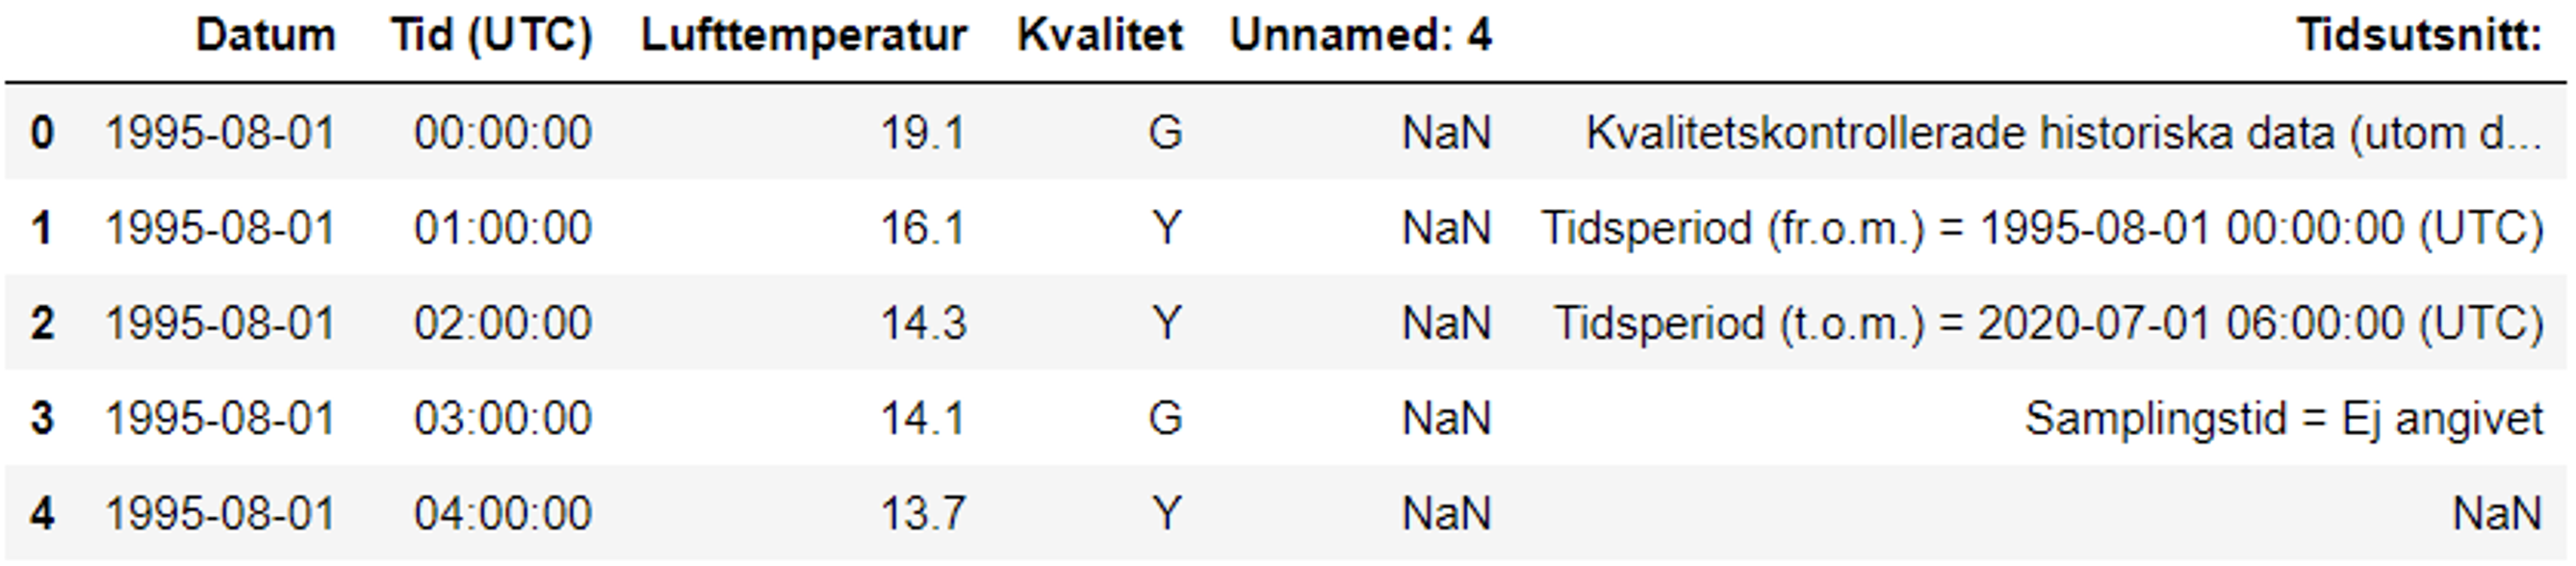
\includegraphics[width=\textwidth]{figures/anaconda9.png}\\
    För mig varnade Jupyter att vissa kolumner innehöll olika typer av data, men jag väljer att strunta i detta eftersom jag endast är intresserad av kolumnerna \textbf{Datum} och \textbf{Lufttemperatur}.
\end{enumerate}
\item \textbf{Grovrensa datan.} Vi skall som ovan ta bort lite kolumner som vi inte behöver, enligt ovan väljer jag att göra en kopia av datan, jag har kvar orginaldatan så jag kan återgå till den om det behövs. I skarpa \emph{Big Data}-sammanhang är detta ofta inte möjligt eftersom datamängden kan vara så pass stora, men i det här fallet är det fullt möjligt. Gör ett mindre dataset med bara de intressanta kolumnerna, \textbf{Datum}, \textbf{Tid}, och \textbf{Lufttemperatur} och kalla den \verb+tempdata+ eller liknande. Ta hjälp av instruktionerna ovan, använd funktionen \verb+columns+ och kom ihåg att första kolumnen är nummer 0. 
    \item \textbf{Börja nosa på datan.} Använd kommandona \verb+describe()+ och \verb+shape+ på din nya dataframe, \verb+tempdata+, för att få en uppfattning om datan och för att säkerställa att rätt kolumner är borttagna.  Via kommandot \verb+describe()+ får jag redan info att medeltemperaturen är ca \SI{8.7}{\celsius} för hela perioden, alla dagar de senaste 25 åren och alla tider på dygnet strax utanför Helsinborg.
    \item \textbf{Banta datan till att bara innehålla månaden juli.} Finns som för många programmeringsproblem väldigt många olika sätt att göra detta, jag har valt att först göra om våra datum som är sparade som text till datum-objekt, så Python/Pandas vet att detta är datum och inte text. Jag lägger till en kolumn i en dataframe genom att ge den ett nytt namn och sedan använder jag funktionen \verb+to_datetime()+ för att göra om från text (sträng) till datum (datetime-objekt). Följande bör fungera:
    \begin{minted}{python}
tempdata["dateobj"] = pd.to_datetime(tempdata["Datum"])        
    \end{minted}
    Vad som görs ovan är att på vänster sida om ”=” skapas en ny kolumn som heter \verb+dateobj+ och det som stoppas in där är från kolumnen \textbf{Datum} konverterat till riktigt datumformat med kommandot \verb+to_datetime()+.\\
    För att hitta de som innehåller juli (månad sju) kan vi konvertera våra datum-objekt till index, som vi ger till \verb+loc[]+ för att hitta rätt, detta låter kanske komplicerat men raden nedan väljer ut alla juli-mätvärden:
\begin{minted}{python}
tempdata.loc[pd.DatetimeIndex(tempdata["dateobj"])==7]
\end{minted}        
Här får ni göra som ni vill, lättast är att skapa en ny variabel som innehåller julidata, lägg till nytt variabelnamn och ”=” precis innan på raden ovan för detta. En vääääldigt användbar funktion för att snabbt sortera i pandas är \verb+.groupby()+ som snabbt som vinden sorterar på årtal eller liknande. Prova gärna denna, vi kommer i sista delen att använda oss av SMHI-datan för att öva lite enkel maskininlärning.
\item \textbf{Redovisa medeltemperatur i juli.} Nu är vi ganska nära slutmålet, med \verb+describe()+ på vårt nya dataset med bara juli med får vi medletemperaturen i juli de senaste 23 åren i fallet med Helsingborg A. Du skall på din inlämning redovisa följande saker:
\begin{enumerate}
    \item Medeltemperatur för juli
    \item Vilka år detta gäller för
    \item Hur många datapunkter det baseras på (count från \verb+describe()+)
    \item Vilken väderstation som har stått för datan som du baserat din analys på.
\end{enumerate}

    \item \textbf{För de snabba (behövs i nästa labb).} Gör en snygg plot av medeltemperaturen i juli för varje år i ditt dataset. Här rekommenderas starkt att använda \verb+.groupby()+ med lämpliga villkor. 
\end{enumerate}

\subsection{Visualisering av data}
TBD.




\end{document}